\documentclass{VUMIFInfKursinis}
\usepackage{algorithmicx}
\usepackage{algorithm}
\usepackage{algpseudocode}
\usepackage{amsfonts}
\usepackage{amsmath}
\usepackage{bm}
\usepackage{color}
\usepackage{graphicx}
% \usepackage{hyperref}  % Nuorodų aktyvavimas
\usepackage{url}

\usepackage{gensymb}
\usepackage{acro}
\usepackage{tikz}
\usetikzlibrary{decorations.pathreplacing}
\usepackage{amssymb,amsthm}
\usepackage[version=4]{mhchem}

\setlength{\jot}{8px} 

% Titulinio aprašas
\university{Vilniaus universitetas}
\faculty{Matematikos ir informatikos fakultetas}
\institute{Informatikos institutas}  % Užkomentavus šią eilutę - institutas neįtraukiamas į titulinį
\department{Programų sistemų katedra}
\papertype{Kursinis darbas}
\title{Medžiagų maišymo modeliavimas cheminėse
reakcijose}
\titleineng{Modelling the mixing of reagents in
chemical reactions}
\status{4 kurso 3 grupės studentas}
\author{Arnas Vaicekauskas}
% \secondauthor{Vardonis Pavardonis}   % Pridėti antrą autorių
\supervisor{Asist. Dr. Rokas Astrauskas}
\date{Vilnius \\ \the\year}

% Nustatymai
% \setmainfont{Palemonas}   % Pakeisti teksto šriftą į Palemonas (turi būti įdiegtas sistemoje)
\bibliography{bibliografija} 

\DeclareAcronym{yag}{
  short   = YAG,
  long    = Itrio aliuminio granatas    
}

\begin{document}
\maketitle

\tableofcontents

\sectionnonum{Sąvokų apibrėžimai}

\begin{itemize}
\item Stoichiometrinis mišinys - tai toks mišinys, kuriame medžiagų proporcijos yra tokios, kokių reikia, kad jos reakcijos metu visiškai sureaguotų
\end{itemize}

% Sutartinių ženklų, simbolių, vienetų ir terminų sutrumpinimų sąrašas (jeigu
% ženklų, simbolių, vienetų ir terminų bendras skaičius didesnis nei 10 ir
% kiekvienas iš jų tekste kartojasi daugiau nei 3 kartus).

\sectionnonum{Įvadas}

% TODO parašyti įvadą

% tyrimo objektas - yag reakcija
% temos aktualumas - aktualu nes yag lazeriai placiai naudojami
% darbo tikslas - yra
% siekiami rezultatai - yra

% tyrimo objektas - yra tiriama matematinis yag reakcijos modelis

% Matematiniai cheminių reakcijų modeliai padeda geriau suprasti veikia 

Itrio aliuminio granato \acs{yag} kristalai legiruoti su neodimio arba kitų lantanoidų jonais yra naudojami kaip kietakūnių lazerių aktyviosios terpės dėl savo geidžiamų optinių savybių. Šios medžiagos lazeriai yra dažnai taikomi gamybos ir medicinos srityse \cite{dubeyExperimentalStudyNd2008, valentiUseErYAG2021}. Šiai medžiagai sintezuoti yra žinoma keletas būdų, tačiau kietafazės reakcijos metodas yra lengviausiai pritaikomas pramoninei gamybai \cite{bhattacharyyaMethodsSynthesisY3AI5O122007, zhangNovelSynthesisYAG2005}. Praktikoje, \acs{yag} sintezė, kietafazės reakcijos metodu, užtrunka mažiausiai kelias valandas priklausomai nuo temperatūros, kurioje vykdomas atkaitinimo procesas \cite{mackeviciusCloserLookComputer2012}. Yra žinoma, kad chemikai bando spartinti šią reakcija periodiškai išmaišydami reagentus. Ivanauskas et al \cite{ivanauskasModellingSolidState2005} pasiūlė matematinį kietafazės \acs{yag} reakcijos modelį ir nustatė reakcijos greičio ir difuzijos konstantas prie tam tikrų temperatūrų, tačiau šis modelis nemodeliuoja minėto išmaišymo proceso. Kompiuterinis modelis, apimantis išmaišymo procesą, galėtų padėti efektyviau suprasti kokią įtaką maišymas turi šiam procesui ir jo trukmei.

Šio \textbf{darbo tikslas} yra sukurti kompiuterinį \acs{yag} reakcijos maišymo modelį ir jį ištirti.

Iškelti darbo uždaviniai:

\begin{enumerate}
\item Sukurti kompiuterinį \acs{yag} reakcijos modelį
\item Patikrinti kompiuterinio modelio rezultatų korektiškumą
\item Papildyti kompiuterinį modelį su maišymo procesu
\item Ištirti kompiuterinio modelio rezultatus
\end{enumerate}

\section{\acs{yag} reakcijos matematinis modeliavimas}

\subsection{\acs{yag} sintezė}

\acs{yag} milteliai gali būti sintezuojami keleta skirtingų būdų: Zolis-Gelis procesu, nusodinimu, solvoterminiu procesu, terminio purškimo procesu bei kietafaze reakcija, kuri lieka viena dažniausiai taikomų dėl savo paprastumo bei galimybės pritaikyti masinei gamybai \cite{zhangNovelSynthesisYAG2005}.

\subsection{Kietafazė reakcija}

Šiame darbe yra modeliuojama paskutinė kietafazės reakcijos stadija, kurios metu reaguodami itrio ir aliuminio oksidai sudaro itrio aliuminio granato kristalus arba tiesiog \acs{yag}:
\begin{align*}
  \ce{3Y_2O_3 + 5Al_2O_3 -> 2Y_3Al_5O_12}
\end{align*}

Prieš pradedant reakciją metalų oksidai yra sutrinami iki smulkiagrūdžių miltelių. Metalų oksidų mišinys yra nuolat kaitinamas 1600\degree C laipsnių temperatūroje ir periodiškai maišomas. Eksperimentiniu būdu išmatuota,kad individualių dalelių turiai prie 1600\degree C temperatūros siekia apie $\sqrt{10}\mu\text{m}^3$ \cite{ivanauskasComputationalModellingYAG2009}.

\begin{figure}[h]
  \centering
  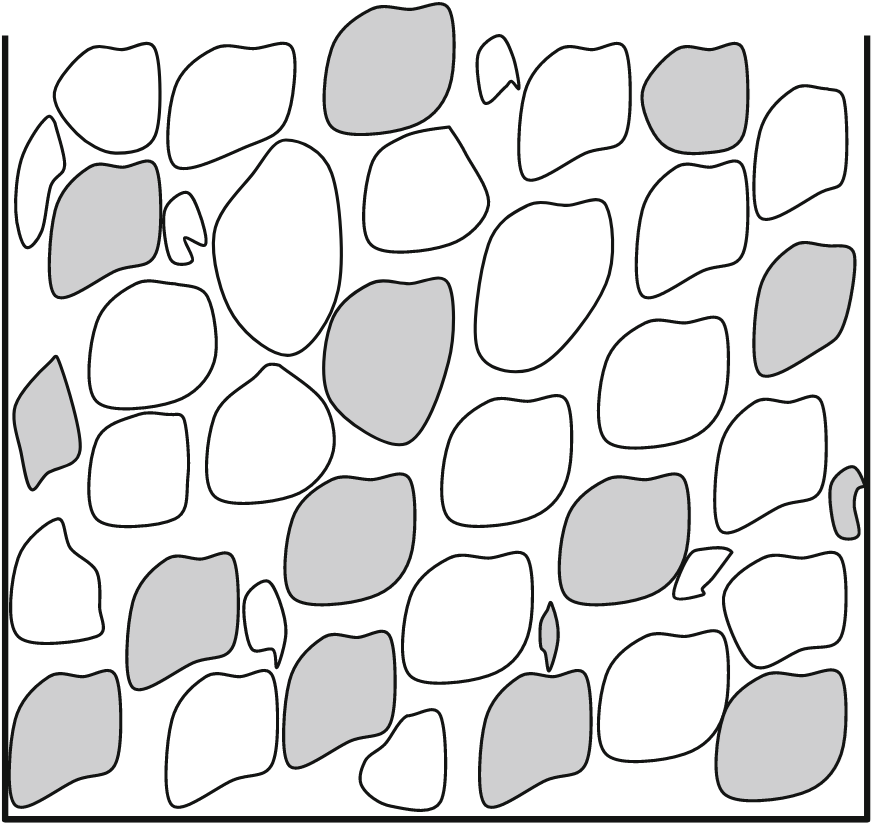
\includegraphics[width=0.25\linewidth]{assets/metal_oxides_mixture.png}
  \label{fig:metal-oxides-mixuter}
  \caption{Priartinto metalų oksidų mišinio iliustracija \cite{}}
\end{figure}

Modeliavimo 

Tokioje temperatūroje metalų oksidai lydosi ir vyksta difuzija, dėl šios priežasties cheminei reakcija yra modeliuojama su difuzijos-reakcijos sistema.

\section{Matematinis modelis}

\subsection{Bedimensis modelis}

\begin{subequations} \label{nodim}
    \begin{align}
    \frac{\partial c_1}{\partial t}&=-3c_1c_2+D\Delta c_1 \label{nodim1}\\
    \frac{\partial c_2}{\partial t}&=-5c_1c_2+D\Delta c_2 \label{nodim2}\\
    \frac{\partial c_3}{\partial t}&=2c_1c_2
    \end{align}
\end{subequations}

kur $c_1,c_2,c_3$ yra bedimensė medžiagų koncentracija, 
$\Delta$ - Laplaso operatorius, $t$ - laikas, 
$D$ - bedimensis medžiagų $c_1$ ir $c_2$ difuzijos koeficientas. Modeliui yra taikoma kraštinė sąlygą:

\begin{equation} \label{general-boundary-cond}
  \nabla c_k(\textbf{x}, t)\cdot\vec{n}=0, \textbf{x}\in\partial\Omega
\end{equation}

Čia $\nabla c_k$ yra medžiagos $c_k$ gradientas, $\textbf{x}$ - erdvės koordinatė, $\partial\Omega$ - simuliuojamos erdvės srities paviršius, o $\vec{n}$ - simuliuojamos erdvės paviršiaus normalė.

\subsection{Elementų maišymasis dviejose dimensijose}

Interpretavus bedimensį modelį \eqref{nodim} dviejose dimensijose gauname lygtis

\begin{subequations} \label{rect}
    \begin{align}
    \frac{\partial c_1}{\partial t}&=-3c_1c_2+D\left(\frac{\partial^2c_1}{\partial x^2}+\frac{\partial^2c_1}{\partial y^2}\right)\\
    \frac{\partial c_2}{\partial t}&=-5c_1c_2+D\left(\frac{\partial^2c_2}{\partial x^2}+\frac{\partial^2c_2}{\partial y^2}\right)\\
    \frac{\partial c_3}{\partial t}&=2c_1c_2
    \end{align}
\end{subequations}

\newpage
Šiam modeliui yra taikomos stoichiometrinės pradinės sąlygos:

% pradinės sąlygos medžiagų koncentracijai turėtų aprašyti stoichiometrinį mišinį

\begin{equation} \label{intial-cond}
  \begin{aligned}
  c_1(x, y, 0) &= \begin{cases} 3c_0, & \text{jei } x \in A \\ 0, & \text{kitaip} \end{cases}\\
  c_2(x, y, 0) &= \begin{cases} 5c_0, & \text{jei } x \notin A \\ 0, & \text{kitaip} \end{cases}\\
  c_3(x, y, 0) &= 0,\\ 
  (x, y) &\in \Omega, \quad\Omega=[0,W]\times[0,H],\quad A=\left[0,\tfrac{W}{2}\right]\times\left[0,\tfrac{H}{2}\right] \cup \left[\tfrac{W}{2},W\right]\times\left[\tfrac{H}{2},H\right].
\end{aligned}
\end{equation}

Čia $c_0$ yra kažkoks teigiamas dydis, kuris nusako pradinę kiekvienos medžiagos koncentraciją sistemoje.

\begin{figure}[h!]
  \centering
  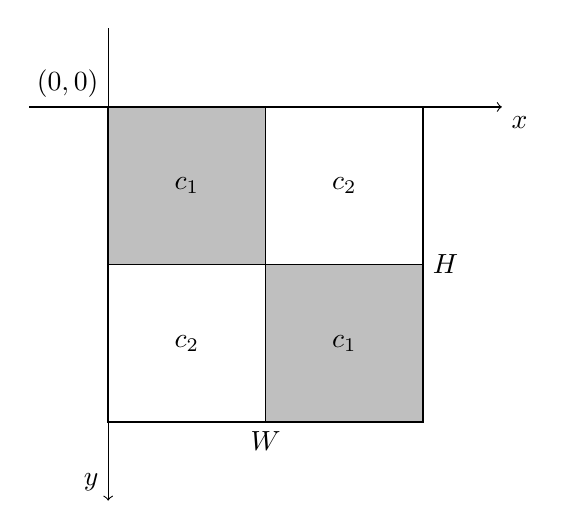
\begin{tikzpicture}[scale=2.0]
      \draw[fill=white] (0,0) rectangle (1,1);
      \draw[fill=white] (1,1) rectangle (2,2);
      \draw[fill=gray!50] (0,1) rectangle (1,2);
      \draw[fill=gray!50] (1,0) rectangle (2,1);
      
      % Draw the boundary of the square
      \draw[thick] (0,0) rectangle (2,2);
  
      % Draw axes
      \draw[->] (-0.5,2) -- (2.5,2) node[anchor=north west] {$x$};  % x-axis
      \draw[<-] (0,-0.5) node[anchor=south east] {$y$} -- (0,2.5);  % y-axis
  
      % Mark the origin
      \node[anchor=south east] at (0,2) {$(0, 0)$};
      
      % Mark the side length L
      \draw[-] (2,0) -- (2,2) node[midway, right] {$H$};
      \draw[-] (0,0) -- (2,0) node[midway, below] {$W$};
      \draw (0.5, 1.5) node[anchor=center] {$c_1$};
      \draw (1.5, 0.5) node[anchor=center] {$c_1$};
      \draw (1.5, 1.5) node[anchor=center] {$c_2$};
      \draw (0.5, 0.5) node[anchor=center] {$c_2$};
  \end{tikzpicture}
  \caption{Sistemos pradinės sąlygos}
\end{figure}

kraštinės sąlygos \eqref{general-boundary-cond} dviejose dimensijose virsta:

\begin{equation} \label{boundary-cond}
\begin{split}
\frac{\partial c_1}{\partial x}\Big|_{x=0}&=\frac{\partial c_1}{\partial x}\Big|_{x=L}=\frac{\partial c_2}{\partial x}\Big|_{x=0}=\frac{\partial c_2}{\partial x}\Big|_{x=L}=0, \quad y\in[0,H], \quad t\in[0,T]\\
\frac{\partial c_1}{\partial y}\Big|_{y=0}&=\frac{\partial c_1}{\partial y}\Big|_{y=L}=\frac{\partial c_2}{\partial y}\Big|_{y=0}=\frac{\partial c_2}{\partial y}\Big|_{y=L}=0, \quad x\in[0,W],\quad t\in[0,T]
\end{split}
\end{equation}

kur $L$ - bedimensis kubo kraštinės ilgis, $T$ - bedimensė proceso trukmė.

\section{Skaitinis modelis}

\subsection{Erdvės diskretizavimas Dekarto koordinačių sistemoje}

Dviejų dimensijų skaitiniam modeliui erdvė buvo padalinta į $N \times M$ taškų 
nutolusių vienas nuo kito fiksuotais $\Delta x$ ir $\Delta y$ atstumais.

\begin{figure}[!h]
\centering
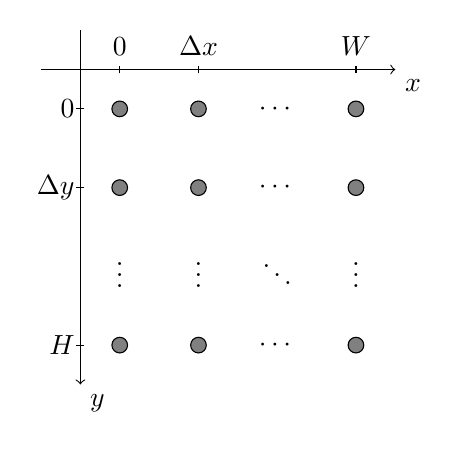
\begin{tikzpicture}

   % Set up styles for the grid
  \tikzset{
    node/.style={circle, draw, fill=gray, inner sep=2pt},
    ellipsis/.style={draw=none, fill=none}
  }

  \draw[->] (0, -0.5) -- (4.5, -0.5) node[anchor=north west] {$x$};  % x-axis
  % x-axis ticks
  \draw[-] (1, -0.55) -- (1, -0.45) node[anchor=south] {$0$};
  \draw[-] (2, -0.55) -- (2, -0.45) node[anchor=south] {$\Delta x$};
  \draw[-] (4, -0.55) -- (4, -0.45) node[anchor=south] {$W$};
  
  \draw[<-] (0.5,-4.5) node[anchor=north west] {$y$} -- (0.5, 0);  % y-axis
  % y-axis ticks
  \draw[-] (0.45, -1) -- (0.55, -1) node[anchor=east] {$0$};
  \draw[-] (0.45, -2) -- (0.55, -2) node[anchor=east] {$\Delta y$};
  \draw[-] (0.45, -4) -- (0.55, -4) node[anchor=east] {$H$};


  % Draw the 3x3 grid of colored circles in a 4x4 layout
  \foreach \x in {1, 2, 4} {
    \foreach \y in {1, 2, 4} {
      \node[node] at (\x, -\y) {};
    }
  }

  % Add ellipses in the 4th row and column for continuation

  \node[ellipsis] at (3, -1) {$\cdots$};
  \node[ellipsis] at (3, -2) {$\cdots$};
  \node[ellipsis] at (3, -4) {$\cdots$};

  \node[ellipsis] at (1, -3) {$\vdots$};
  \node[ellipsis] at (2, -3) {$\vdots$};
  \node[ellipsis] at (4, -3) {$\vdots$};

  \node[ellipsis] at (3, -3) {$\ddots$};

\end{tikzpicture}
\caption{ diskretizuota erdvė }
\end{figure}

Čia 

\subsection{Dviejų dimensijų skaitinis modelis Dekarto koordinačių sistemoje}

Remiantis išreikštiniu baigtinių skirtumų metodu iš dvimačio modelio galima gauti skaitinį modelį.
\begin{subequations} \label{numerical-eqs}
\begin{align}
\frac{c^{n+1}_{1,i,j}-c^n_{1,i,j}}{\Delta t}&=
-3c^{n}_{1,i,j}c^{n}_{2,i,j}\notag\\
&+D\left(\frac{c^n_{1,i-1,j}-2c^n_{1,i,j}+c^n_{1,i+1,j}}{(\Delta x)^2}+\frac{c^n_{1,i,j-1}-2c^n_{1,i,j}+c^n_{1,i,j+1}}{(\Delta y)^2}\right)\\
\frac{c^{n+1}_{2,i,j}-c^n_{2,i,j}}{\Delta t}&=
-5c^{n}_{1,i,j}c^{n}_{2,i,j}\notag\\
&+D\left(\frac{c^n_{2,i-1,j}-2c^n_{2,i,j}+c^n_{2,i+1,j}}{(\Delta x)^2}+\frac{c^n_{2,i,j-1}-2c^n_{2,i,j}+c^n_{2,i,j+1}}{(\Delta y)^2}\right)\\
\frac{c^{n+1}_{3,i,j}-c^n_{3,i,j}}{\Delta t}&=2c^{n}_{1,i,j}c^{n}_{2,i,j},
\end{align}
\end{subequations}

kur $n\in[0, T)$ - laiko momentas, 
$i\in[0,N)$ - diskrečios erdvės taško koordinatė $x$ ašyje,
$j\in[0,M)$ - diskrečios erdvės taško koordinatė $y$ ašyje,
$c^n_{1,i,j}$ - pirmos medžiagos kiekis diskrečios erdvės taške $i$, $j$ laiko momentu $n$,
$c^n_{2,i,j}$ - antros medžiagos kiekis diskrečios erdvės taške $i$, $j$ laiko momentu $n$,
$c^n_{3,i,j}$ - trečios medžiagos kiekis diskrečios erdvės taške $i$, $j$ laiko momentu $n$,
$\Delta t$ - laiko žingsnis,
$\Delta x$ - diskrečios erdvės žingsnis $x$ ašimi,
$\Delta y$ - diskrečios erdvės žingsnis $y$ ašimi.

\subsection{Modelio skaitinis stabilumas}

Norint užtikrinti skaitinį programos stabilumą, reikia užtikrinti, kad visais laiko momentais, visuose diskretizuotos erdvės taškuose, visų medžiagų koncentracijos išliktų ne neigiamos. Parodysime, kad tai užtikrinti, užtenka pasirinkti pakankamai mažą laiko žingsnį $\Delta t$. Pirmiausia įvedame porą konstantų:
\begin{align*}
\mu_x = \frac{D\Delta t}{(\Delta x)^2}, \quad
\mu_y = \frac{D\Delta t}{(\Delta y)^2}
\end{align*}

Tada pertvarkome dviejų dimensijų skaitinį modelį \eqref{numerical-eqs} taip, kad kairėse lygčių pusėse liktų medžiagų koncentracija laiko momentu $n+1$, o dešinėse lygčių pusėse sugrupuojame narius pagal medžiagų koncentracija skirtinguose diskretizuotos erdvės taškuose:

\begin{subequations} \label{eqs:r-coefs}
    \begin{align}
    c^{n+1}_{1,i,j}&=\underbrace{(1-3\Delta tc^{n}_{2,i,j}-2(\mu_x+\mu_y))}_{R_1}c^n_{1,i,j}+\mu_xc^n_{1,i-1,j}+\mu_xc^n_{1,i+1,j}+\mu_yc^n_{1,i,j-1}+\mu_yc^n_{1,i,j+1} \label{r-coefs1}\\
    c^{n+1}_{2,i,j}&=\underbrace{(1-5\Delta tc^{n}_{1,i,j}-2(\mu_x+\mu_y))}_{R_2}c^n_{2,i,j}+\mu_xc^n_{2,i-1,j}+\mu_xc^n_{2,i+1,j}+\mu_yc^n_{2,i,j-1}+\mu_yc^n_{2,i,j+1} \label{r-coefs2}\\
    c^{n+1}_{3,i,j}&=c^n_{3,i,j}+2\Delta tc^{n}_{1,i,j}c^{n}_{2,i,j} \label{r-coefs3}
    \end{align}
\end{subequations}

Baziniu atveju, kai $n=0$, medžiagų koncentracija visuose taškuose yra ne neigiama, kaip numatyta pradinėje sąlygoje \eqref{intial-cond}. Darome indukcijos hipotezės prielaidą, kad medžiagų koncentracija visuose diskretizuotos erdvės taškuose, laiko momentu $n$ bus ne neigiama:

\begin{align} \label{induction-assumption}
    c^n_{k,i,j} \geqslant 0, \quad k=1,2,3,\quad i=0,1,\dots,N-1,\quad j=0,1,\dots,M-1
\end{align}

Akivaizdu, kad lygtyje \eqref{r-coefs3}, medžiagos koncentracija $c^{n+1}_{3,i,j}$ negali tapti neigiama dėl prielaidos \eqref{induction-assumption} ir fakto, kad $\Delta t>0$. Pirmos medžiagos lygtyje \eqref{r-coefs1}, galima pastebėti, kad dėmenys su medžiagų koncentracijomis iš aplinkinių diskretizuotos erdvės taškų visada bus ne neigiami dėl prielaidos \eqref{induction-assumption} ir fakto, kad $\mu_x>0$ ir $\mu_y>0$:

\begin{align*}
    \mu_xc^n_{1,i-1,j}+\mu_xc^n_{1,i+1,j}+\mu_yc^n_{1,i,j-1}+\mu_yc^n_{1,i,j+1}\geqslant 0
\end{align*}

Taigi $c^{n+1}_{1,i,j}$ ženklą lemia tik koeficientas $R_1$, todėl įvedame ribojimą, kad $R_1\geqslant 0$. Analogiškai, iš antros medžiagos lygties \eqref{r-coefs2} gauname, kad $R_2\geqslant 0$ ir turime nelygybių sistemą:

\begin{align} \label{impl-ineqs}
  \begin{cases}
    1-3\Delta tc^{n}_{2,i,j}-2(\mu_x+\mu_y)\geqslant 0\\
    1-5\Delta tc^{n}_{1,i,j}-2(\mu_x+\mu_y)\geqslant 0
  \end{cases}, \quad i=0,1,\dots,N-1, \quad j=0,1,\dots,M-1
\end{align}

Išreiškę nelygybes \eqref{impl-ineqs} per laiko žingsnį $\Delta t$ gauname:

\begin{align} \label{dt-ineq}
  \begin{cases}
    \Delta t \leqslant (3c^{n}_{2,i,j}+2D((\Delta x)^{-2}+(\Delta y)^{-2}))^{-1}\\
    \Delta t \leqslant (5c^{n}_{1,i,j}+2D((\Delta x)^{-2}+(\Delta y)^{-2}))^{-1}
  \end{cases}
\end{align}

Gautas nelygybes galima apjungti dėl jų panašios struktūros. Norint, kad apjungta nelygybė tenkintų sistemą \eqref{dt-ineq}, reikia išrinkti mažiausią įmanomą laiko žingsnį $\Delta t$, o taip bus tada, kai trupmenos vardiklis bus kuo įmanoma didesnis. Dėl to gauta nelygybė įgaus formą:

\begin{align}
  \Delta t \leqslant \left(\max(3c^{n}_{2,i,j}, 5c^{n}_{1,i,j})+2D\left((\Delta x)^{-2}+(\Delta y)^{-2}\right)\right)^{-1}
\end{align}

Taigi parodėme, kad išvengti neigiamų sprendinio reikšmių, užtenka pasirinkti pakankamai mažą laiko žingsnį $\Delta t$. Tačiau čia sustoti būtų nenaudinga, nes turime rekursyvią priklausomybę -- norint pasirinkti $\Delta t$, reikia žinoti maksimalią medžiagų reikšmę simuliacijoje, o jai sužinoti reikia atlikti simuliaciją su pasirinktu laiko žingsniu $\Delta t$.

Parodysime, kad galima panaikinti laiko žingsnio priklausomybę nuo laiko momento $n$ ir kad $\Delta t$ priklauso tik nuo pradinių sąlygų $c^0_{1,i,j}$ ir $c^0_{2,i,j}$. Medžiagos kiekio pokytis per laiką sistemoje gali būti apskaičiuoti taip:

\begin{align}
  \frac{\partial q_k}{\partial t} = \int_\Omega \frac{\partial c_k}{\partial t} dA
\end{align}

Įstatom bedimensio modelio lygtis \eqref{nodim1}, \eqref{nodim2}:

\begin{align}
  \frac{\partial q_1}{\partial t}=-3\int_\Omega c_1c_2\,dA + \int_\Omega \Delta c_1\,dA=-3\int_\Omega c_1c_2\,dA + \int_\Omega \nabla \cdot (\nabla c_1)\,dA\\
  \frac{\partial q_2}{\partial t}=-5\int_\Omega c_1c_2\,dA + \int_\Omega \Delta c_2\,dA=-5\int_\Omega c_1c_2\,dA + \int_\Omega \nabla \cdot (\nabla c_2)\,dA
\end{align}

\newpage
Pagal Gauso divergencijos teoremą ir kraštinę sąlygą \eqref{general-boundary-cond} gauname, kad:

\begin{align}
\int_\Omega \nabla \cdot (\nabla c_k) dA = \int_{\partial\Omega} \nabla c_k \cdot \vec{n}\, ds = 0,\quad k=1,2
\end{align}

Todėl pirmos ir antros medžiagų kiekio pokytis per laiką bus ne teigiamas:

\begin{align}
  \frac{\partial q_1}{\partial t}=-3\int_\Omega c_1c_2\,dA \leqslant 0\\
  \frac{\partial q_2}{\partial t}=-5\int_\Omega c_1c_2\,dA\leqslant 0
\end{align}

Tai reiškia, kad maksimalios pirmos ir antros medžiagų reikšmės bus laiko momente $n=0$, tad nelygybę galime suprastinti iki šios formos:

\begin{align}
  \Delta t \leqslant \left(\max(3c^{0}_{2,i,j}, 5c^{0}_{1,i,j})+2D\left((\Delta x)^{-2}+(\Delta y)^{-2}\right)\right)^{-1}
\end{align}

Laiko žingsnis čia vis dar priklauso nuo diskretizuotos erdvės koordinatės $(i, j)$, tačiau tai nesunku pastebėti, kad užtenka parinkti didžiausią reikšmę iš kiekvienos pradinės sąlygos -- tokiu būdu laiko žingsnis gausis mažiausias. Iš pradinės sąlygos \eqref{intial-cond} turime:

\begin{align*}
\max c^0_{1,i,j}=3c_0,\quad i=0,1,\dots,N-1, \quad j=0,1,\dots,M-1\\
\max c^0_{2,i,j}=5c_0,\quad i=0,1,\dots,N-1, \quad j=0,1,\dots,M-1
\end{align*}

Taigi, kad simuliacija išliktų skaitiškai stabili, reikia, kad laiko žingsnis $\Delta t$ tenkintų šią nelygybę.

\begin{align*}
  \Delta t \leqslant \left(15c_0+2D\left((\Delta x)^{-2}+(\Delta y)^{-2}\right)\right)^{-1}
\end{align*}


\section{Programos sudarymas ir rezultatai}

Pagal dviejų dimensijų skaitinį modelį \eqref{numerical-eqs} sudarytas uždavinį sprendžiantis skriptas ir kiti pagalbiniai skriptai duomenims vaizduoti ir tikrinti. Skriptai rašomi \textit{Python} programavimo kalba, naudojant \textit{NumPy}, \textit{SciPy}, \textit{Matplotlib} paketus. 

Modelio rezultatai yra saugomi kaip atskiri \textit{.npy} formato failai, kurie yra skirti saugoti \mbox{\textit{NumPy}} masyvus. Dėl praktinių rezultatų panaudojimo ir tyrimo nebūtina saugoti informacijos apie visus laiko žingsnius, todėl išsaugotuose rezultatų failuose, simuliacijos kadrai laiko kryptimi gali būti praretinti iki tūkstančio kartų, priklausomai nuo pasirinktų parametrų. Pagalbiniai duomenų vaizdavimo skriptai šiuos duomenis agreguoja į grafikus, kurie išsaugomi \textit{.png} formatu.

\begin{figure}[h!]
\centering
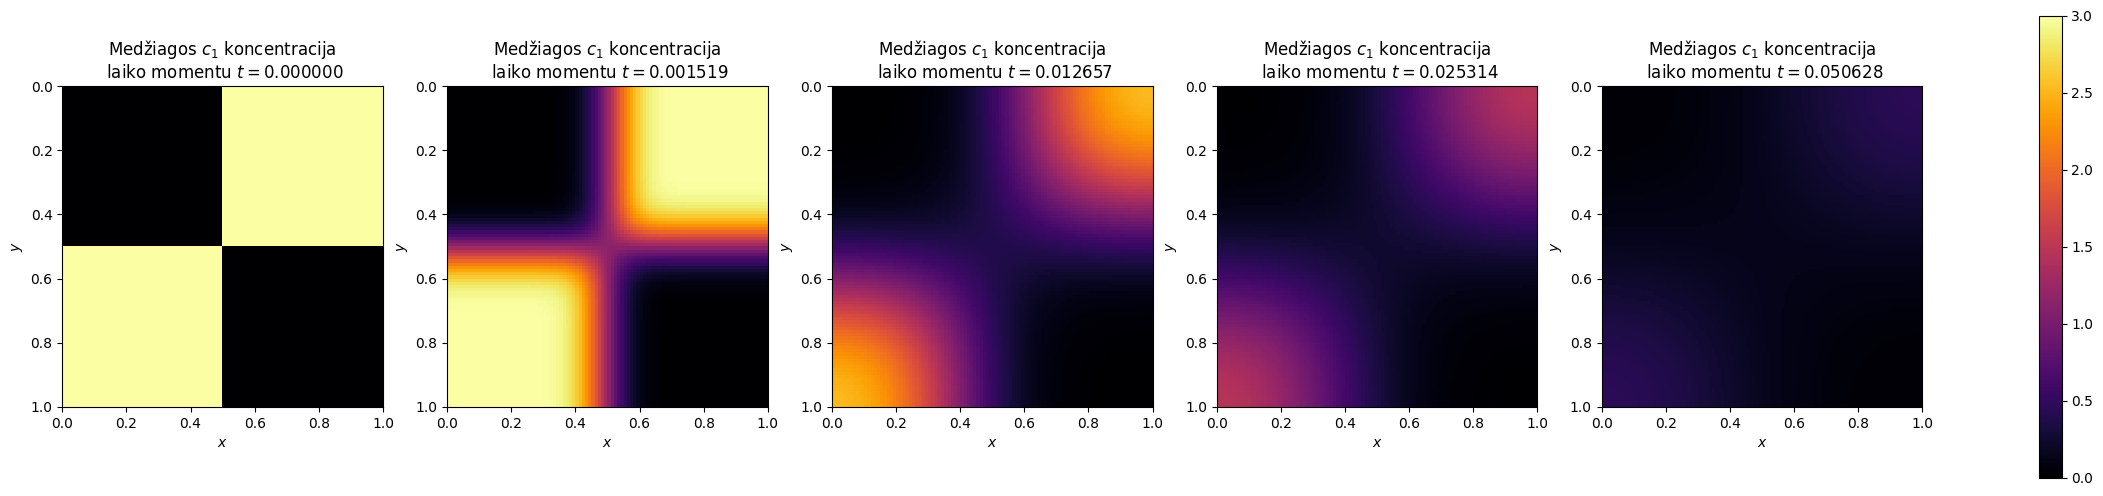
\includegraphics[width=\textwidth]{../assets/examples-c1.png} \\
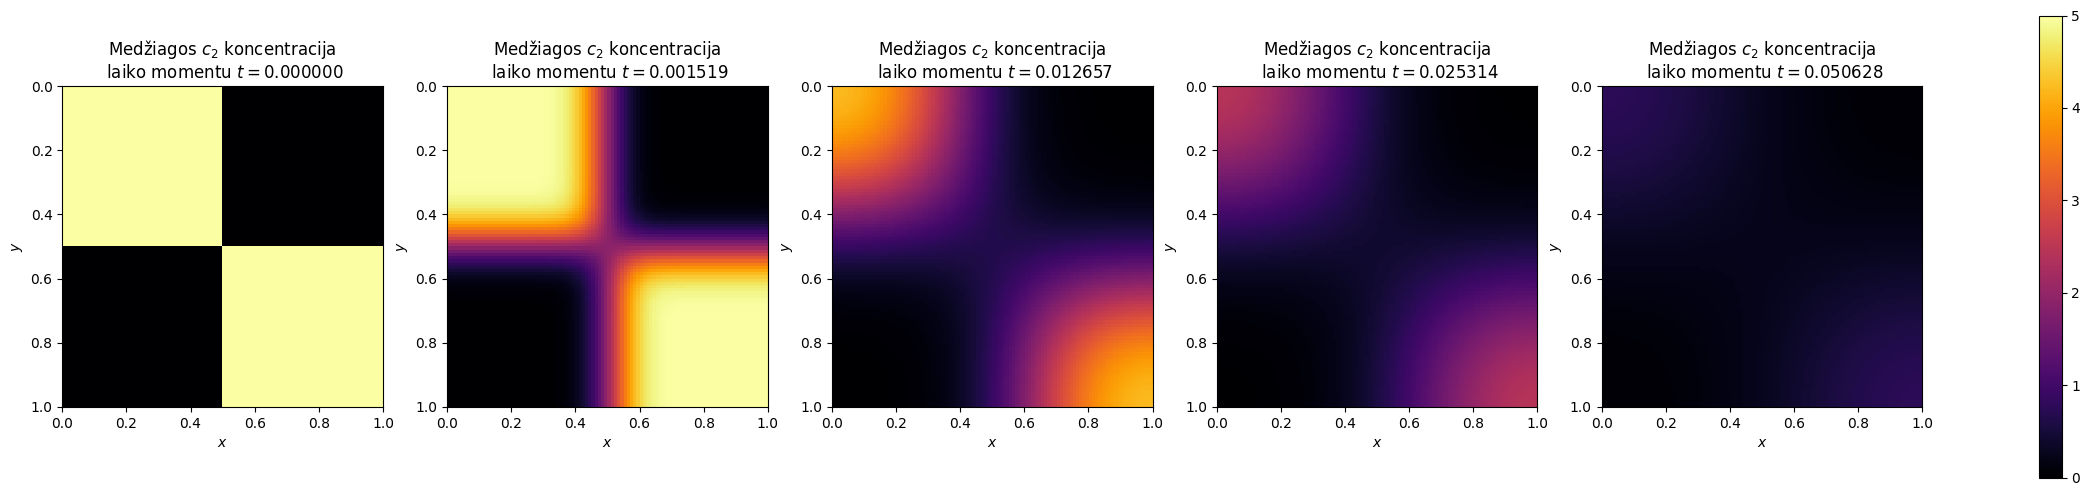
\includegraphics[width=\textwidth]{../assets/examples-c2.png} \\
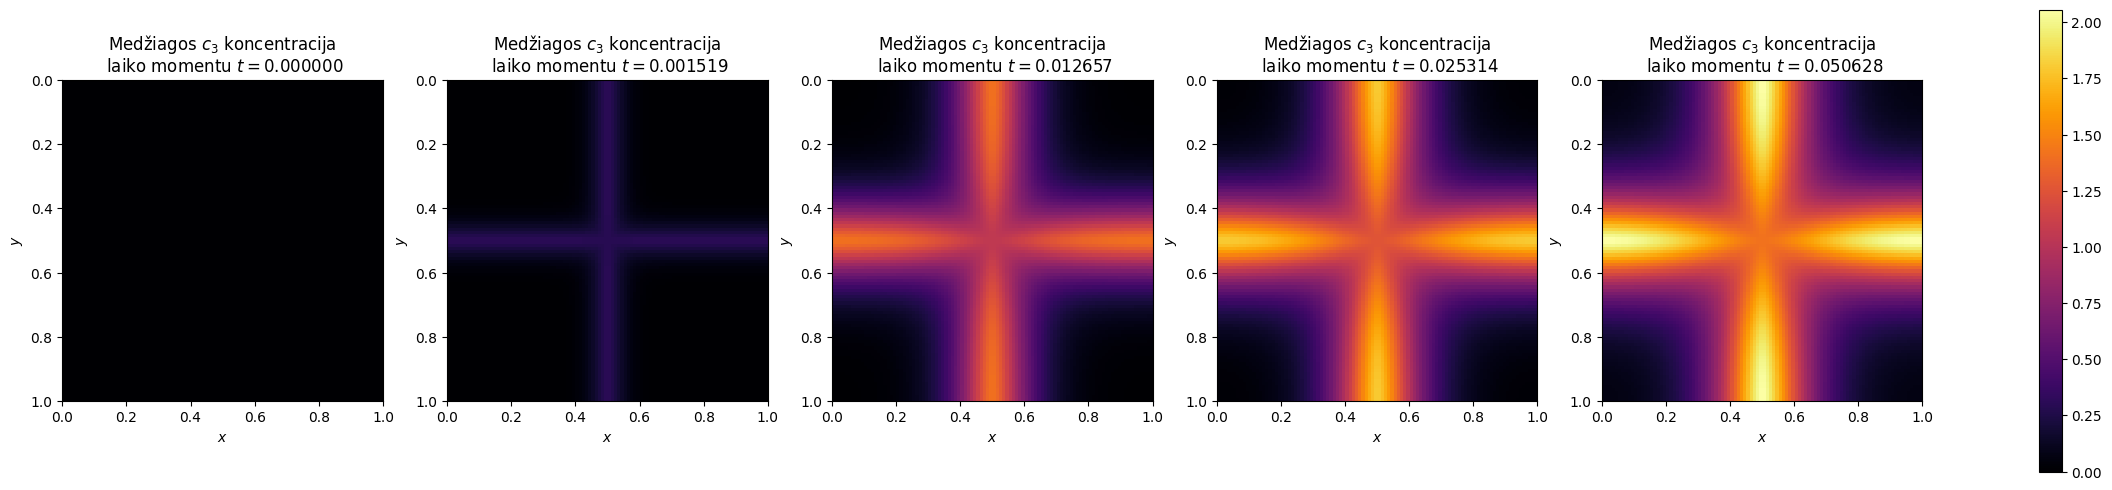
\includegraphics[width=\textwidth]{../assets/examples-c3.png}
\caption{Kompiuterinio modelio rezultato pavyzdys. $D = 0.05$, $W = 1$, $H = 1$, $\Delta x = \frac{1}{99}$, $\Delta y = \frac{1}{99}$, $k = 1$, $c_0 = 1$, $\Delta t$ - pasirinktas pagal \eqref{numerical-stability-condition} }
\label{result-example}
\end{figure}

\newpage
\subsection{Programos korektiškumo tikrinimas}

\subsubsection*{Korektiškumo tikrinimas bendru atveju}

% Čia galima tikrint kad individualiu ląstelių
% - keičiant dx/dy kiekio per laiką sprendinys vizualiai konverguoja
% - kiekio grafikai per laika medžiagom c1 ir c2 mažėja, o c3 - didėja.
% - jei nustatom reakcijos koeficienta k = 0, kiekis bus pastovus
% Tikrinti rezultatų korektiškumui yra naudojami tie patys duomenys kaip ir rezultatų vaizdavimui. 

Nagrinėjant programos korektiškumą naudosime modelio rezultatų duomenis. Dėl didelės rezultatų dimensijos būtų sunku interpretuoti grafiškai pavaizduotus sprendinio duomenis, kaip \hbox{\ref{result-example}-ame} pavyzdyje, todėl vietoje tokių grafikų, tyrinėsime medžiagų kiekius sistemoje. Galime išskleisti formulę medžiagos kiekiui bendru atveju \eqref{quantity-general} ir gausime formulę diskrečiam atvejui \cite{strangCalculusVolume32016}:
\begin{align}
    q(t) = \int_\Omega c\,dV = \int_0^W \int_0^H c(x, y, t)\,dy\,dx
\end{align}
Pakeičiam dvigubą integralą su dviguba Rymano suma ir gaunam, kad medžiagos $c_m$ kiekis diskrečiu laiko momentu $n$ yra:
\begin{align}
    q_{m, n}= \sum_{i=0}^{N-1}\sum_{j=0}^{M-1} c_{m, i,j}^n \frac{W\cdot H}{N\cdot M} \quad m=1, 2, 3
\end{align}
Norint nustatyti, ar programa veikia korektiškai galima tikrinti, ar mažinant žingsnių dydį, skaitinis sprendinys artėja prie tikrojo sprendinio. Šiuo atveju mažinsime erdvės žingsnius $\Delta x$ ir $\Delta y$. Tai lemia diskretaus tinklelio taškų kiekio padidėjimą, nes egzistuoja atvirkštinė priklausomybė tarp erdvinių žingsnių dydžio ir diskrečių taškų kiekio atitinkamomis ašimis (\ref{meshx}, \ref{meshy}).
\begin{figure}[h!]
    \centering
    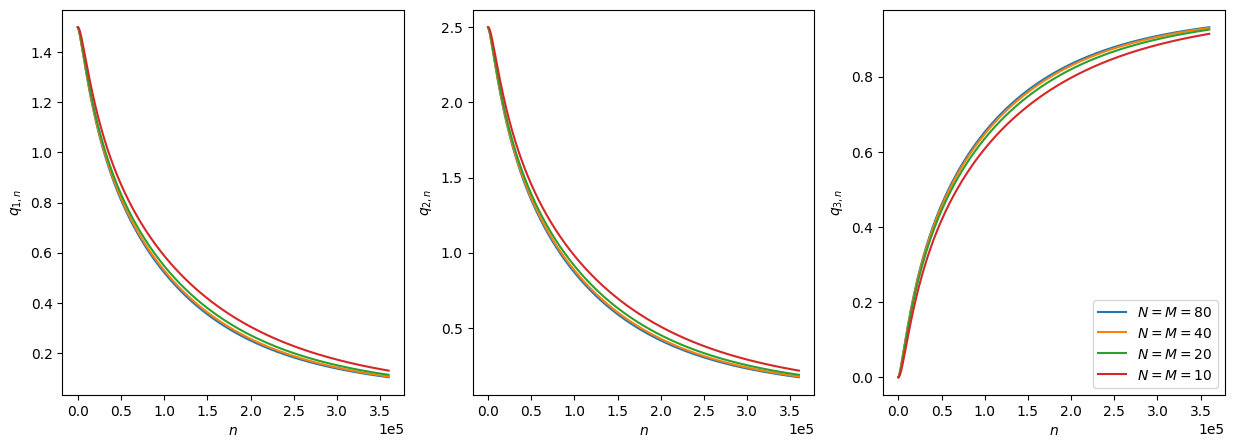
\includegraphics[width=\textwidth]{../assets/space-error-v2.png} \\
    \caption{Kompiuterinio modelio rezultatai - medžiagų kiekių priklausomybė nuo laiko. Čia $\tau=3.6\times 10^5$, $D=0.05$, $W = 1$, $H=1$, $k = 1$, $c_0 = 1$, $\Delta t = 1\times 10^{-5}$, $\Delta x$, $\Delta y$ - kintami ir priklauso nuo $N$ bei $M$ }
    \label{results-space-error}
\end{figure}

\ref{results-space-error}-ame pav. matome, kad eksponentiškai didinant diskrečių taškų skaičių, sprendinių grafikai tolygiai artėja prie sprendinio su didžiausiu tikslumu, darome prielaidą, kad didinant diskrečių taškų skaičių, skaitinis sprendinys konverguoją į tikrąjį sprendinį. Kažkuriuo momentu diskrečios erdvės taškų kiekio didinimas nebeduoda ypatingai didelių rezultato pagerėjimų. Sprendinių grafikuose taip pat galima įžvelgti, kad pirmų dviejų medžiagų kiekiai per laiką griežtai ne mažėja - tai mes teoriškai parodėme \eqref{negative-quantity}, taip, žinoma, yra dėl  medžiagų reakcijos. 

Analogiškai galima būtų fiksuoti erdvinius žingsnius $\Delta x, \Delta y$ ir stebėti kaip keičiasi skaitinis sprendinys mažinant laiko žingsnį $\Delta t$. Dėl priežasčių, kurios vėliau bus akivaizdžios vaizduosime du sprendinius - vienas iš jų gautas pasirinkus $\Delta t$ pagal \eqref{numerical-stability-condition}, o kitam paimta konkreti reikšmė $\Delta t = 10^{-4}$.

\begin{figure}[h!]

\centering

\caption{Kompiuterinio modelio rezultatai - medžiagų kiekių priklausomybė nuo laiko. Čia $\tau=3.6\times 10^5$, $D=0.05$, $W = 1$, $H=1$, $k = 1$, $c_0 = 1$, $\Delta x = \Delta y = 79^{-1}$}

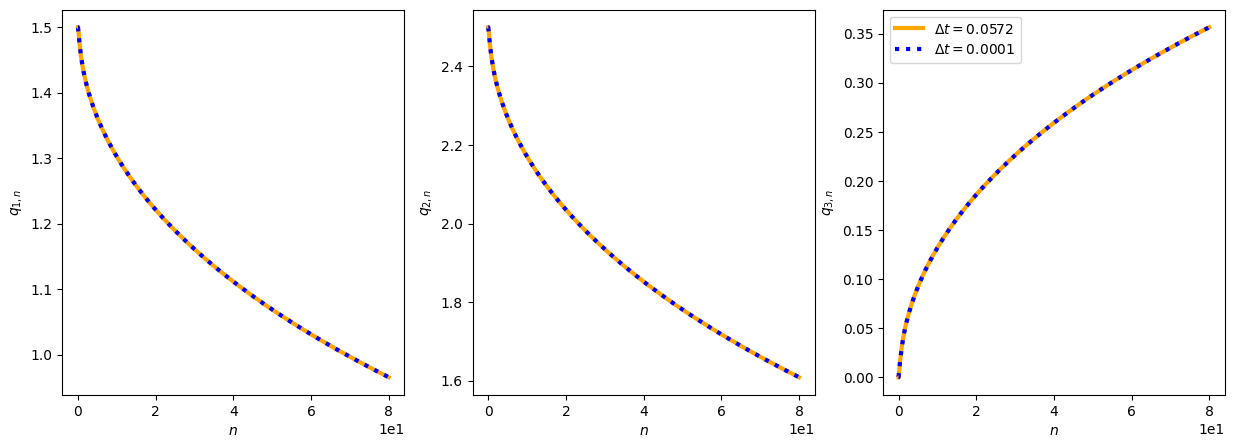
\includegraphics[width=\textwidth]{../assets/time-error-2.png}

\label{time-error}

\end{figure}

\ref{time-error}-ame pav. matome, kad sprendiniai yra identiški. Laiko žingsnio  $\Delta t$ pasirinkimas pagal \eqref{numerical-stability-condition} yra pakankamai geras ir mažesnių laiko žingsnių pasirinkimas neduoda tikslesnių rezultatų.

\newpage

\subsubsection*{Korektiškumo tikrinimas kai vyksta tik difuzija}

Jei reakcijos koeficientas būtų lygus nuliui, vienintelis sistemoje vykstantis procesas būtų pirmų dviejų medžiagų difuzija. Jei skaitinis modelis veikia korektiškai, rezultatuose turėtų būti galima matyti, kad difuzijos metu medžiagos kiekis sistemoje nekinta, tai teoriškai parodėme skyriuje apie skaitinį stabilumą \eqref{no-q-change}.

\begin{figure}[h!]
    \centering
    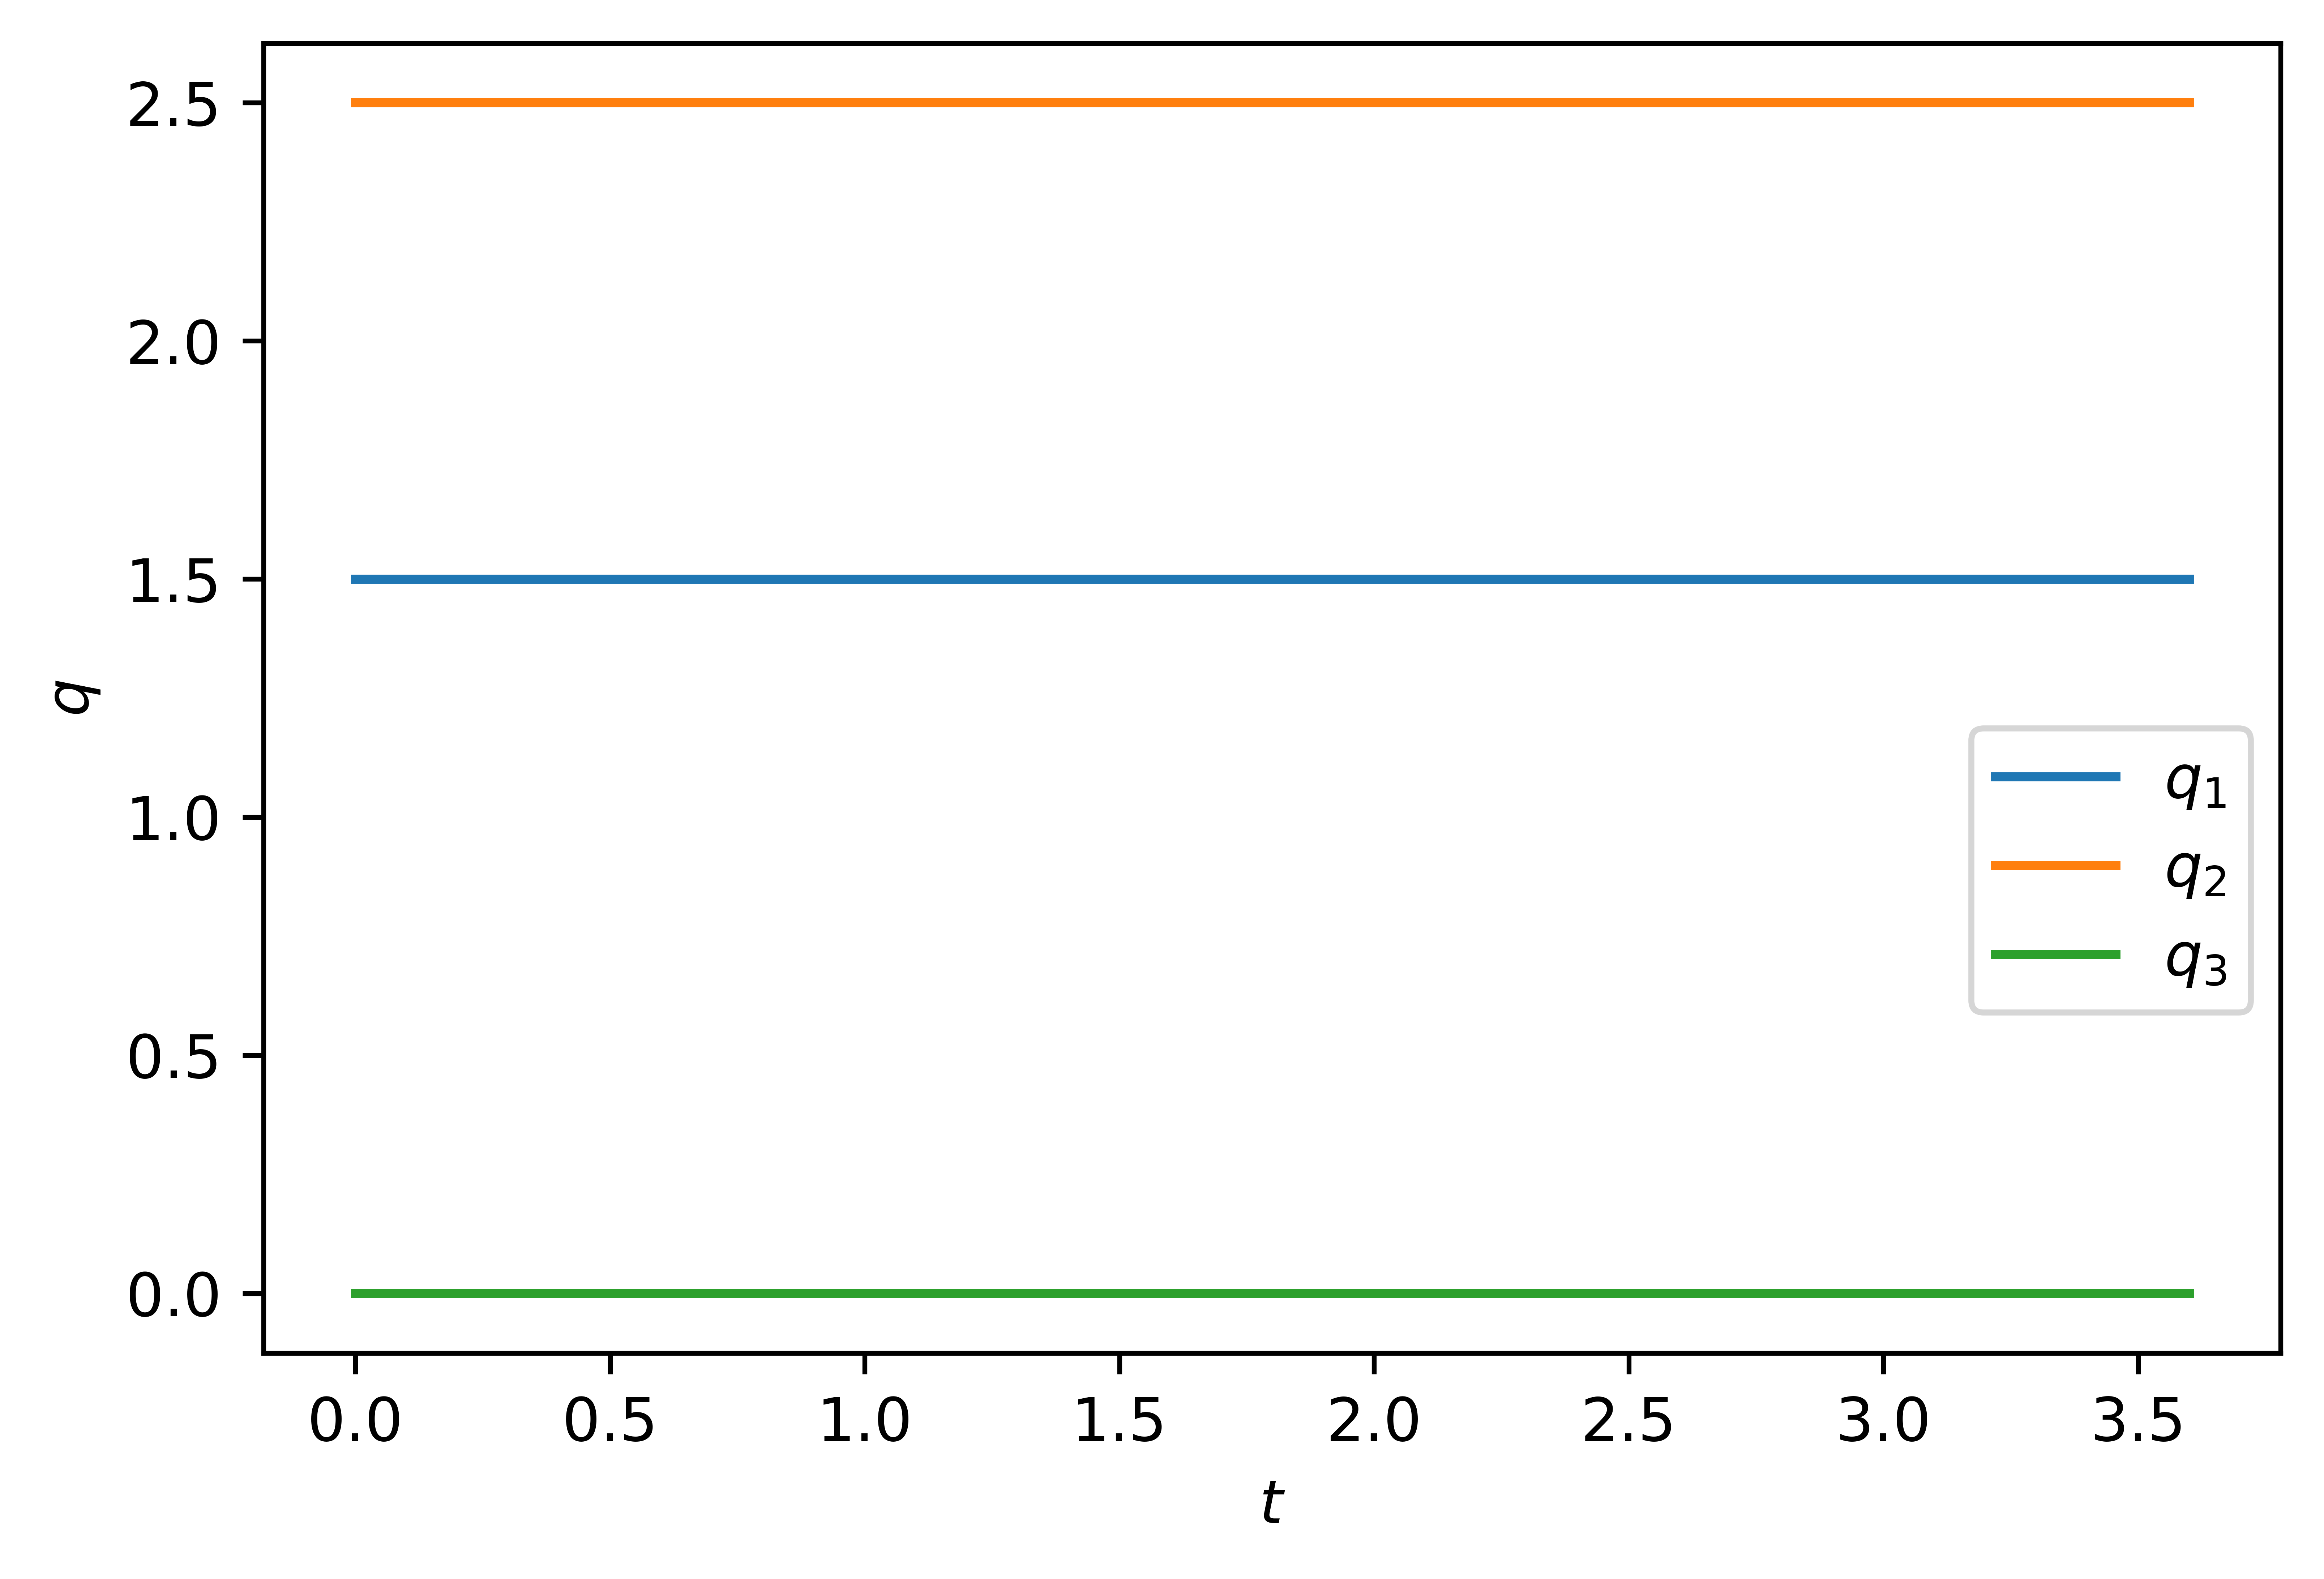
\includegraphics[width=0.5\textwidth]{../assets/no-reaction.png}
    \caption{Kompiuterinio modelio rezultatai - medžiagų kiekių priklausomybė nuo laiko, kai reakcija nevyksta. $D = 0.05$, $W = 1$, $H = 1$, $\Delta x = \frac{1}{79}$, $\Delta y = \frac{1}{79}$, $k = 0$, $c_0 = 1$, $\Delta t = 1\times 10^{-5}$ }
    \label{no-reaction}
\end{figure}

\ref{no-reaction}-ame pavyzdyje kompiuterinės programos rezultatai yra būtent tokie, kokių tikėjomės, tačiau iš šio grafiko negalime užtikrinti, kad simuliacijoje išvis kažkas vyksta. Norint patikrinti, ar medžiagos difunduoja korektiškai galime pabandyti pavaizduoti medžiagų kiekį visoje srityje $\Omega$ kaip rezultatų pavyzdyje \eqref{result-example}.

\begin{figure}[h!]
\centering
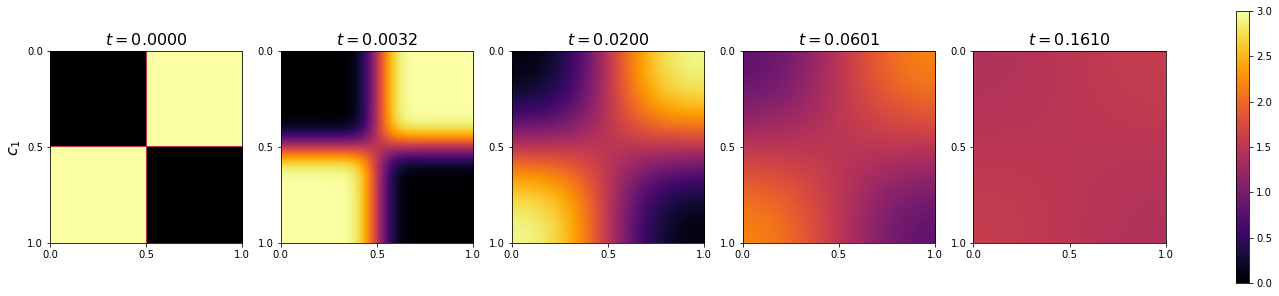
\includegraphics[width=\textwidth]{../assets/only-diffusion-c1.png} \\
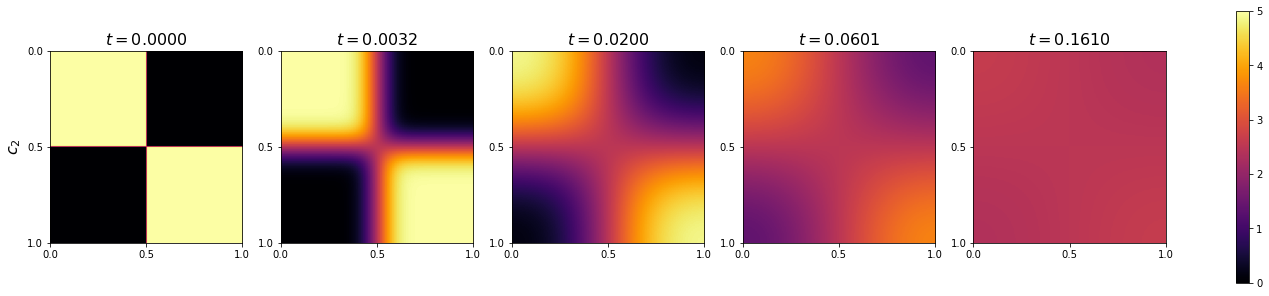
\includegraphics[width=\textwidth]{../assets/only-diffusion-c2.png}
\caption{Kompiuterinio modelio rezultato pavyzdys, kai vyksta tik difuzija. $D = 0.05$, $W = 1$, $H = 1$, $\Delta x = \frac{1}{79}$, $\Delta y = \frac{1}{79}$, $k = 0$, $c_0 = 1$, $\Delta t = 1\times 10^{-5}$ }
\label{only-diffusion}
\end{figure}

Čia akivaizdžiai galime matyti, kad medžiagų difuzija vyksta ir einant laikui medžiagos tolygiai pasiskirsto po erdvę.




\section{Maišymo modeliavimas}
\subsection{Maišymo proceso modelis}

Vykstant reakcijai, chemikai periodiškai ištraukia reagentus iš krosnies, kurioje vyksta reakcija, todėl maišymas vyksta prie daug žemesnės temperatūros. Milteliai yra išmaišomi nepažeidžiant mikrodalelių struktūros - t. y. maišoma taip, kad mikrodalelės neskiltų. Konstruojant kompiuterinį modelį šiam procesui atkreipsime dėmesį į kelias svarbias detales:

\begin{itemize}
    \item Išmaišymas vyksta prie daug žemesnės temperatūros negu reakcija
    \item Išmaišymas gali vykti kelis kartus
    \item Išmaišymo procesas nėra deterministinis
\end{itemize}

\paragraph{Maišymas prie žemesnės temperatūros}

Kadangi maišymas vyksta prie daug žemesnės temperatūros negu pati reakcija, darysime prielaidą, kad ištraukus reagentus iš krosnies cheminė reakcija ir difuzija nevyksta, todėl medžiagų maišymą modeliuosime kaip momentinį procesą, kuris įvyksta tarp diskrečių laiko žingsnių.

\paragraph{Maišymas kelis kartus}

Praktikoje vykdant šią reakcija chemikai savo nuožiūra pasirenka laiką, kuriuo vykdys išmaišymą, todėl ir kompiuterinis modelis turėtų suteikti vartotojui pasirinkimą nurodyti konkrečius laiko momentus, kada vyks medžiagų išmaišymas. Šiuos laikus žymėsime taip:

\begin{align}
    t^1_\text{mix}, t^2_\text{mix}, \dots, t^{T^*}_\text{mix} \quad T^*\in \mathbb{N}
\end{align}

Čia $T^*$ -- bendras išmaišymų skaičius, o $t^i_\text{mix}$ -- $i$-tojo išmaišymo laikas. Kadangi kompiuterinis modelis laiko informaciją apie diskrečius laiko taškus $t_n$, mes negalime tiesiogiai apibrėžti sąlygos, kad išmaišymas vyks konkrečiu laiko momentu $t^i_\text{mix}$, todėl medžiagas išmaišysime einamajame laiko žingsnyje $t_n$, kuris yra artimiausias išmaišymo laikui $t^i_\text{mix}$:

\begin{figure}[!h]
\centering
\caption{Šiuo atveju, išmaišymas įvyks laiko žingsniu $t_n$, o ne $t_{n+1}$, nes $t^i_\text{mix}$ yra arčiau laiko momento $t_n$}
\label{mix-inequality-graphic}
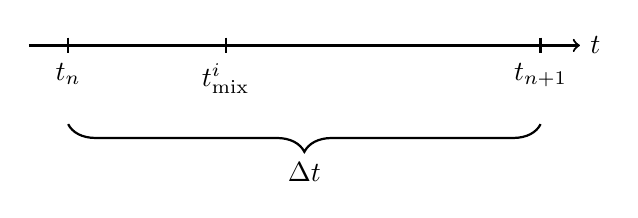
\begin{tikzpicture}[thick]

% Main timeline
\draw[->] (-0.5,0) -- (6.5,0) node[right] {$t$}; % Timeline with axis label

% Time points
\foreach \x/\label in {0/{$t_n$}, 2/{$t^i_\text{mix}$}, 6/{$t_{n+1}$}} {
    \draw (\x,0.1) -- (\x,-0.1) node[below] {\label};
}

% Braces for interval
\draw[decorate,decoration={brace,amplitude=10pt,mirror}] (0,-1) -- (6,-1) node[midway,below=10pt] {$\Delta t$};


\end{tikzpicture}
\end{figure}

arba kitaip sakant išmaišymas įvyks laiko žingsniu $t_n$, jei:

\begin{align}
    \vert t_n - t^i_\text{mix} \vert < \frac{1}{2}\Delta t \label{mix-inequality}
\end{align}

\paragraph{Nedeterministinis maišymas}

Maišymas praktikoje yra chaotiškas procesas, todėl sudarydami kompiuterinį modelį turime į tai atsižvelgti. Maišymą modeliuosime kaip reakcijos erdvės sričių atsitiktinį išdėstymą. Pradinė erdvę $\Omega$ padalinsime į mažesnes, nepersidengiančias, vienodas kvadratines sritis $\Omega_i$:

\begin{figure}[!h]
\centering
\caption{Padalinta reakcijos erdvė $\Omega$}
\label{split-reaction-space}

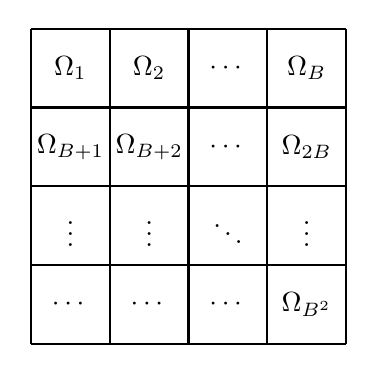
\begin{tikzpicture}
% Draw grid
\draw[thick] (0,0) grid (4,4);

% Row 1
\node at (0.5, 3.5) {$\Omega_1$};
\node at (1.5, 3.5) {$\Omega_2$};
\node at (2.5, 3.5) {$\cdots$};
\node at (3.5, 3.5) {$\Omega_B$};

% Row 2
\node at (0.5, 2.5) {$\Omega_{B + 1}$};
\node at (1.5, 2.5) {$\Omega_{B + 2}$};
\node at (2.5, 2.5) {$\cdots$};
\node at (3.5, 2.5) {$\Omega_{2B}$};

% Row 3
\node at (0.5, 1.5) {$\vdots$};
\node at (1.5, 1.5) {$\vdots$};
\node at (2.5, 1.5) {$\ddots$};
\node at (3.5, 1.5) {$\vdots$};

% Row 4
\node at (0.5, 0.5) {$\cdots$};
\node at (1.5, 0.5) {$\cdots$};
\node at (2.5, 0.5) {$\cdots$};
\node at (3.5, 0.5) {$\Omega_{B^2}$};
\end{tikzpicture}
\end{figure}

Tada sugeneruosime atsitiktinę $B^2$-permutaciją $\sigma: \{ 1, 2, \dots, B^2 \} \to \{ 1, 2, \dots, B^2 \} $ ir $B^2$ atsitiktinių kampų $\theta_i \in \{0, \frac{\pi}{2}, \pi, \frac{3\pi}{2}\}$. Kiekviena iš sričių $\Omega_i$ keliauja į poziciją, kurioje yra sritis $\Omega_{\sigma(i)}$, tačiau pasukta kampu $\theta_i$. Čia, kaip kompiuterinio modelio vartotojai, mes galime pasirinkti sričių kiekio parametrą $B\in\mathbb{N}$, tačiau reikia užtikrinti, kad diskrečių erdvės taškų kiekiai $N, M$ atitinkamomis ašimis būtų dalomi iš $B$. 

Atlikus tokį erdvės sudalinimą, gali atsitikti taip, kad kai kurių sričių $\Omega_i$ kaimynės bus tos pačios medžiagos arba atsisukusios į srities $\Omega$ išorę ir dėl to ties jų sandūra reakcija nevyks. Po išmaišymo tai gali pasikeisti ir galime daryti spėjimą, kad turėtume matyti staigų reakcijos greičio padidėjimą. 

% \paragraph{Neskylančios mikrodalelės}

% Norint atkartoti praktikoje pastebimą faktą, kad išmaišymo metu reagentų mikrodalelės nėra smulkinamos, modeliuodami medžiagų maišymą apsiribojime, kad 


% aprasyti kaip tas maisymas atrodo is tikro ir kaip skiriasi nuo modelio

% matematinis modelis maisymui
% stop salyga

\subsection{Reakcijos stabdymo sąlyga}

Pristatyti kompiuterinio modelio rezultatai rodo, kad vykstant reakcijai, reagentų kiekis erdvėje artėja prie 0, tačiau niekad jo nepasiekia. Tai būdinga ir realybėje vykstančioms reakcijoms, dėl šios priežasties kompiuterinio modelio darbą stabdysime, kai sureaguos $\eta_\text{stop}\%$ pradinių medžiagų kiekio. Matematiškai reakcijos stabdymo laiką $t_\text{stop}$ galime apibrėžti taip:

\begin{align}
    q(t_\text{stop})=\left(1-\frac{\eta_\text{stop}}{100}\right)q(0),\quad \eta_\text{stop}\in[0, 100)
\end{align}

Tolimesniems pavyzdžiams ir analizei naudosime konkrečią reikšmę $\eta_\text{stop}=97$ ir reakciją stabdysime laiku $t_\text{stop}$, kai $q(t_\text{stop})=0.03q(0)$. Toks procentas pasirinktas todėl, kad sureagavus 97\% reagentų, reakcija iš esmės yra pasibaigusi ir gautų duomenų užtenka atlikti analizei.

\newpage
\subsection{Maišymo procesu papildytos programos rezultatų analizė}

\begin{figure}[h!]
\centering
\caption{Kompiuterinio modelio, papildyto išmaišymo procesu, rezultato pavyzdys. Čia $\eta_\text{stop} = 97$, $t^1_\text{mix} = 1h$, $B = 2$, $D = 28\times 10^{-6} \frac{\mu m^2}{s}$, $W = \sqrt[3]{10}\mu m$, $H = \sqrt[3]{10}\mu m$, $k = 0$, $c_0 = 10^{-6} \frac{g}{\mu m^3}$, $\Delta x = \Delta y = \frac{\sqrt[3]{10}}{79} \mu m$ }
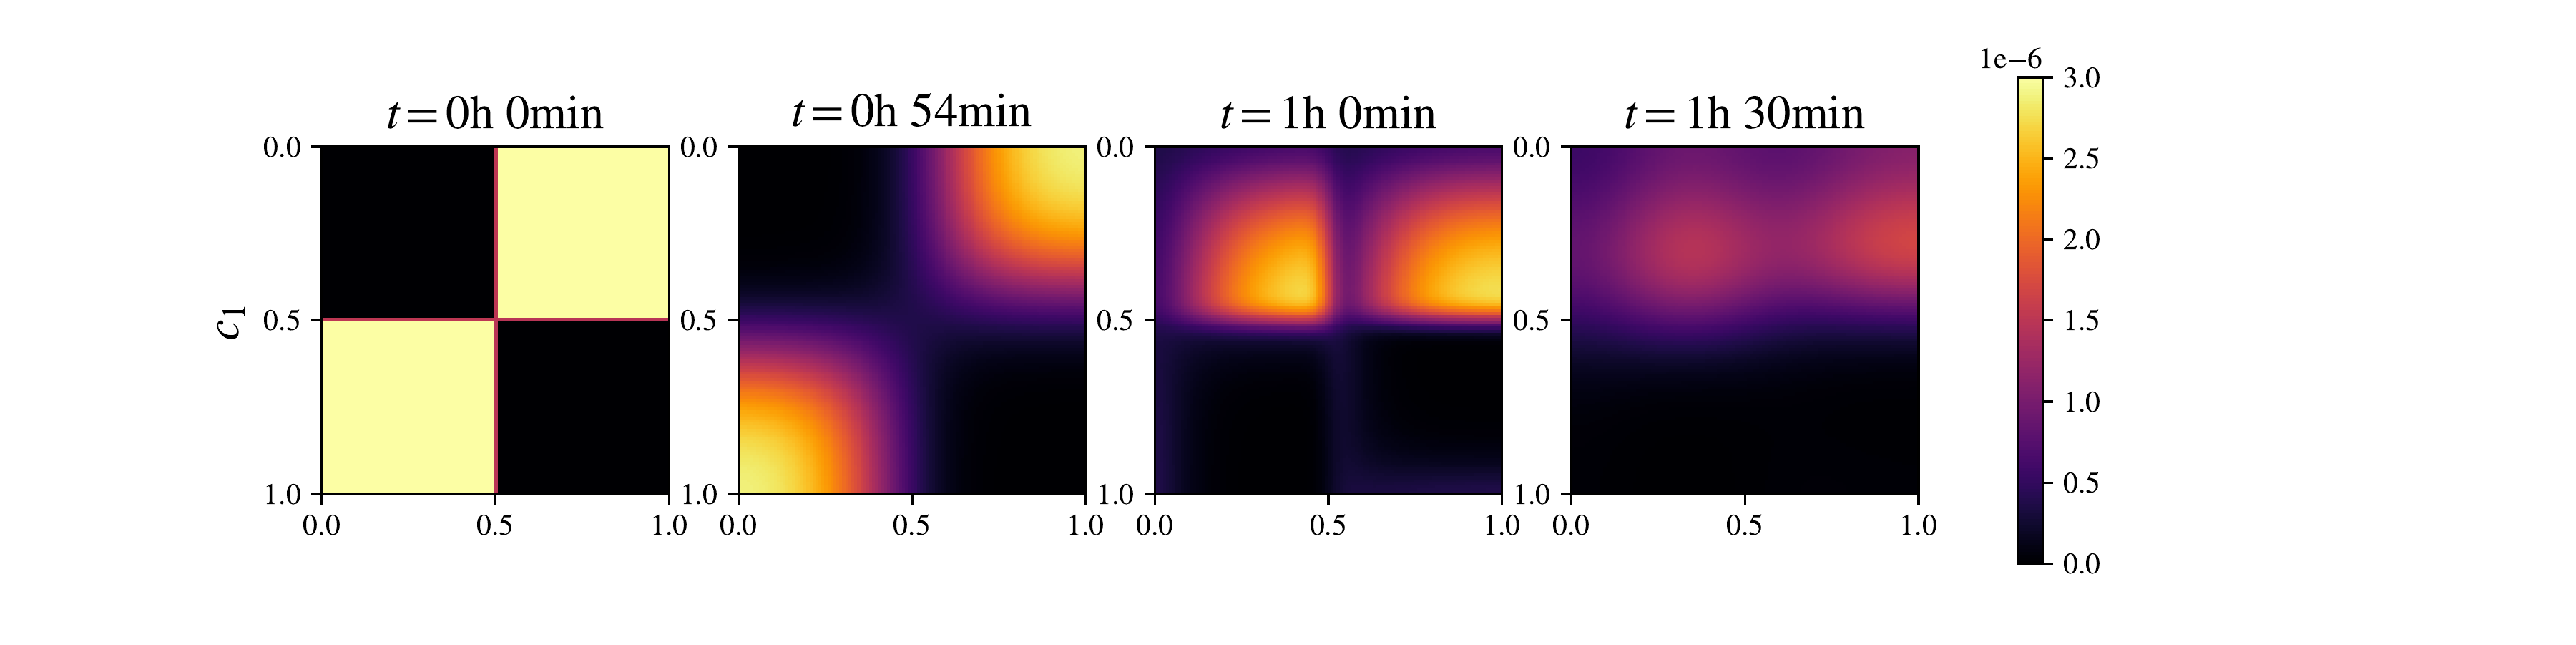
\includegraphics[width=\textwidth]{../paper/assets/random-mix-example-c0-1.png} \\
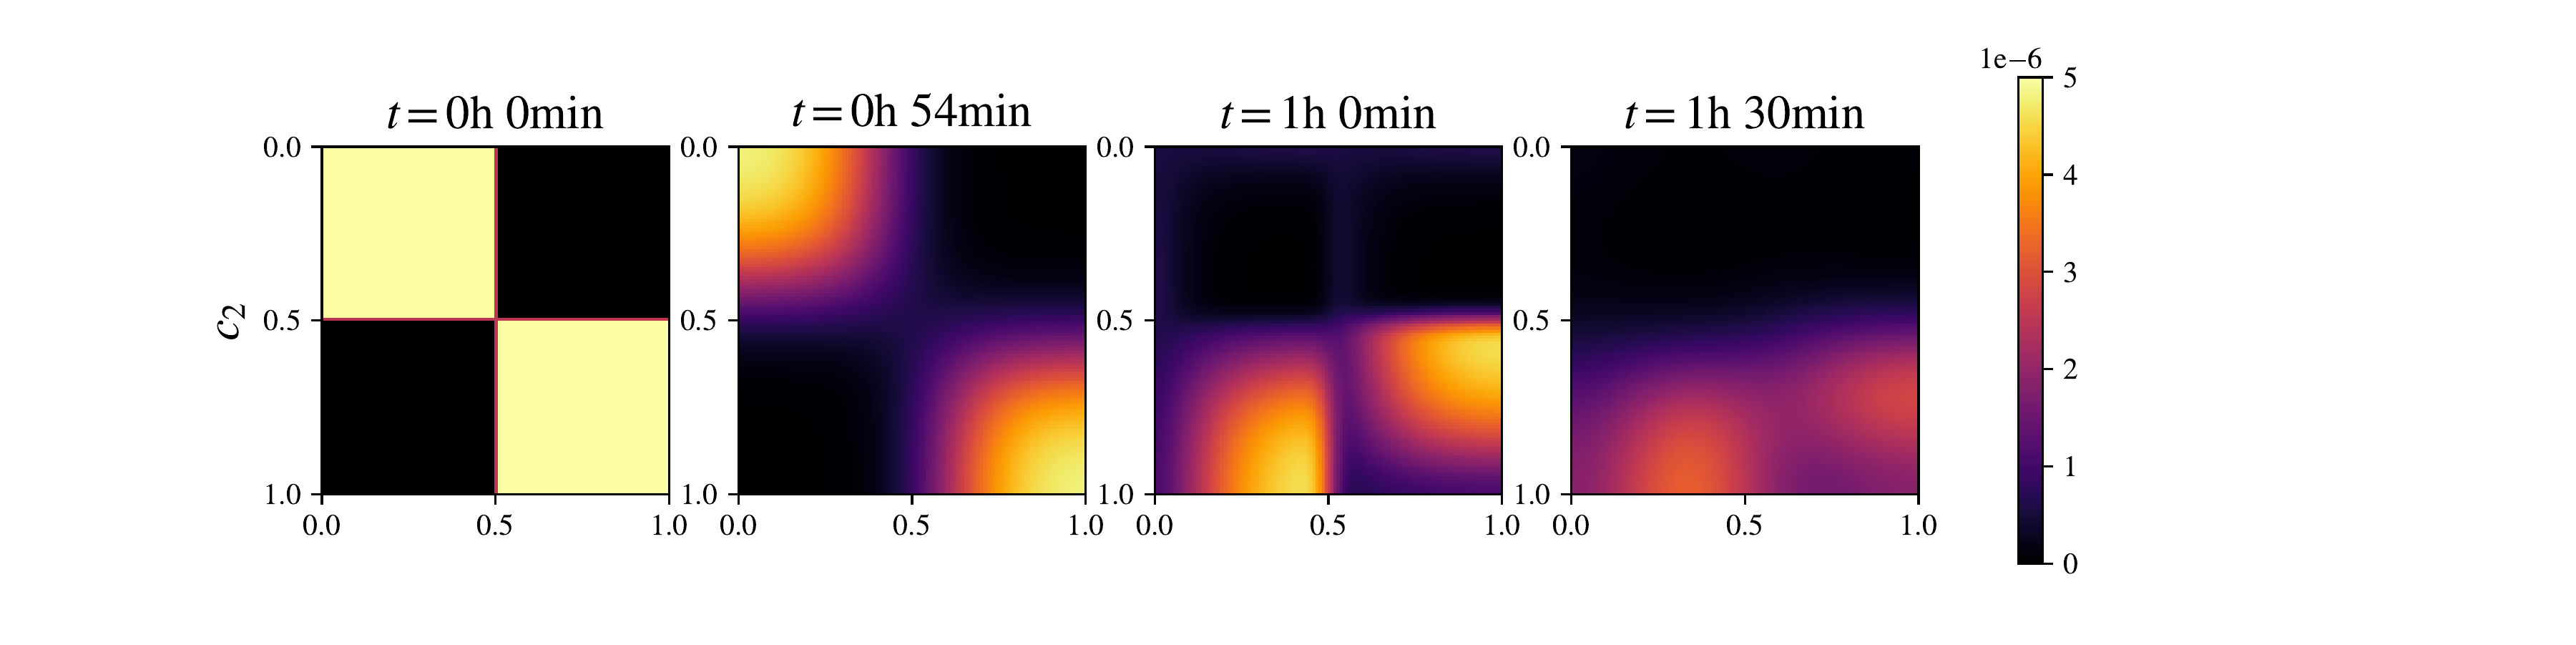
\includegraphics[width=\textwidth]{../paper/assets/random-mix-example-c1-1.png} \\
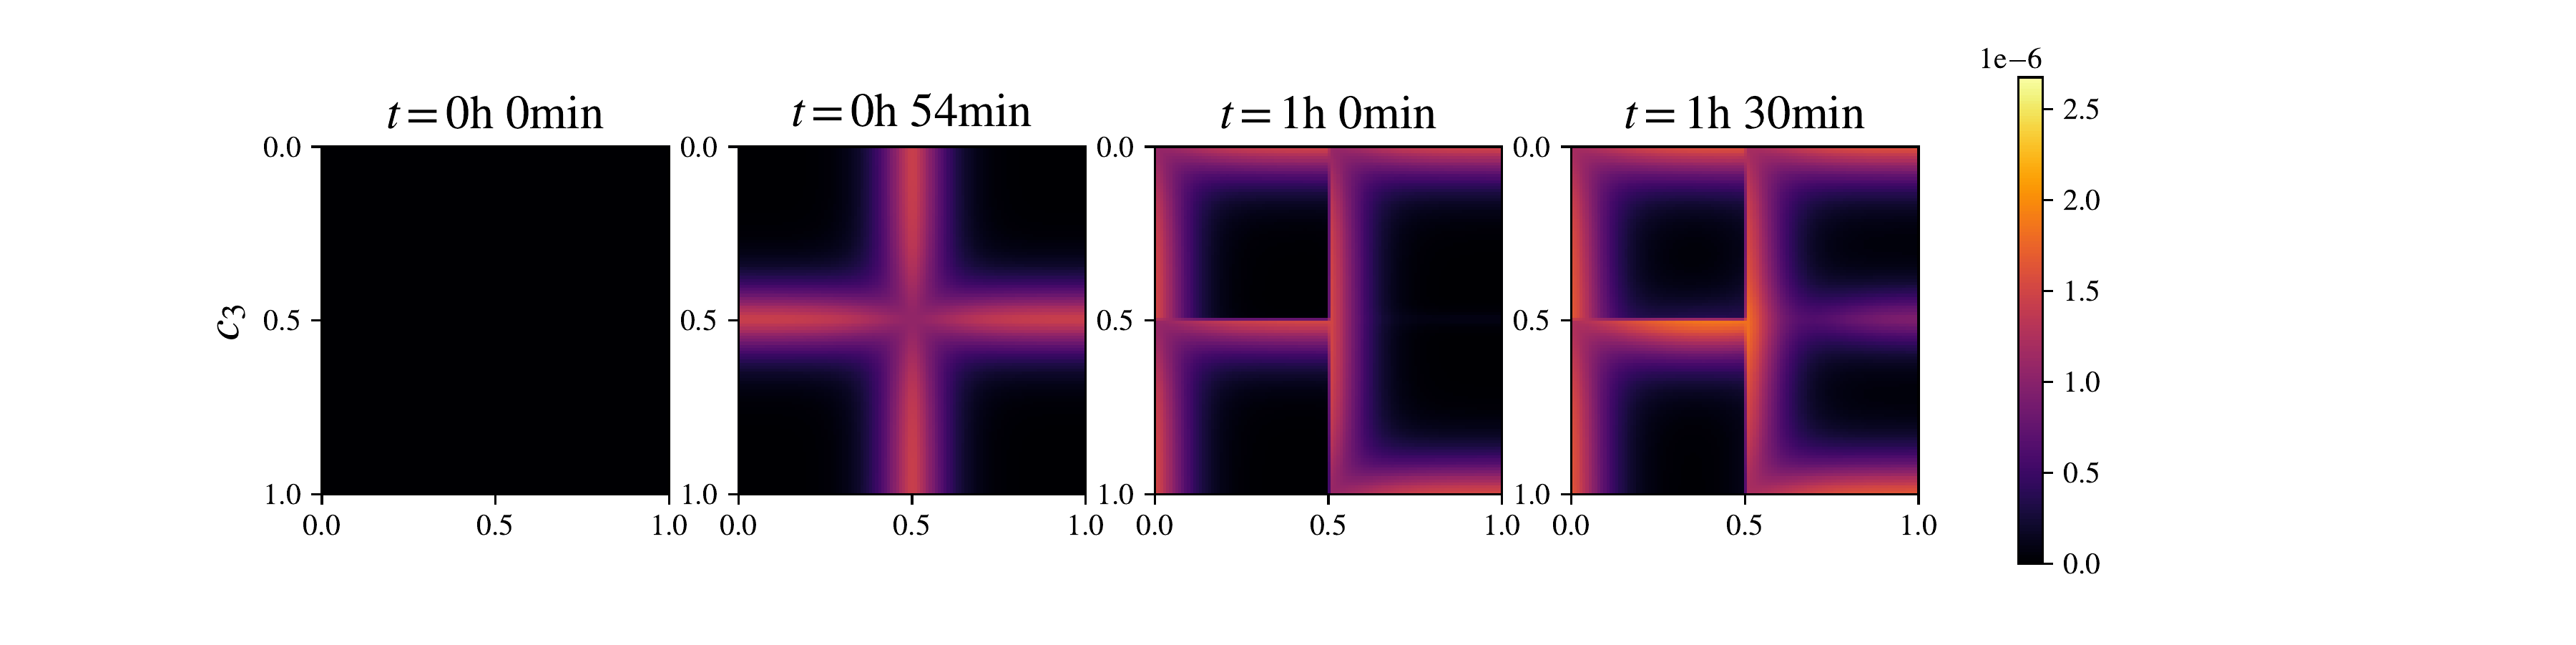
\includegraphics[width=\textwidth]{../paper/assets/random-mix-example-c2-1.png}
\label{mix-example}
\end{figure}

\ref{mix-example}-ame pavyzdyje matome kaip atrodo reakcijos eiga, kada vyksta išmaišymas. Šiuo atveju išmaišymas vyko laiku $t=1h$. Trečias stulpelis vaizduoja reakcijos erdvę ką tik po išmaišymo proceso, kada visos keturios sritys $\Omega_i$ yra atsitiktinai pasukamos ir sumaišomos. Kadangi nuo išmaišymo praejo labai mažai laiko, medžiagos nespėjo sureaguoti ir dėl to matome didelio kontrasto artefaktus ties kai kuriomis išmaišytų sričių kraštinėmis. Čia galime pastebėti tam tikrą problemą su atsitiktiniu išmaišymu - šiuo atveju, po išmaišymo, nesusidūrė prieš tai dar nesureagavusios dalelių kraštinės, todėl reakcijos greičiui šis procesas neturėjo beveik jokios įtakos. Tai gana akivaizdžiai matosi jei pažiūrėtume į medžiagos kiekio grafiką.

\newpage

\begin{figure}[h!]
    \centering
    \caption{Kompiuterinio modelio rezultatų palyginimas su ir be maišymo proceso. Čia $\eta_\text{stop} = 97$, $B = 2$, $D = 28\times 10^{-6} \frac{\mu m^2}{s}$, $W = \sqrt[3]{10}\mu m$, $H = \sqrt[3]{10}\mu m$, $k = 0$, $c_0 = 10^{-6} \frac{g}{\mu m^3}$, $\Delta x = \Delta y = \frac{\sqrt[3]{10}}{79} \mu m$ }
    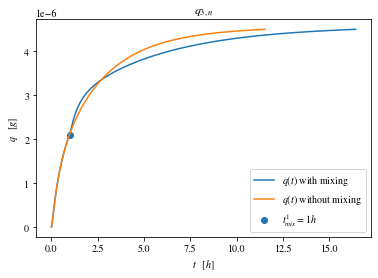
\includegraphics[width=0.5\textwidth]{../paper/assets/bad-mix-qnt-compare.png}
    \label{bad-mix-qnt-example}
\end{figure}

\ref{bad-mix-qnt-example}-ame pavyzdyje puikiai matosi, kad išmaišymas nepagreitino reakcijos, o ją sulėtino. Praktiniuose eksperimentuose taip niekad nenutinka todėl, kad mikrodalelių skaičius yra pakankamai didelis ir toks atvejis tampa beveik neįmanomas. Šiuo atveju galėtume pakeisti 

% Prie bendro atvejo apie stabdymo salyga parasyti konkretu, kuri po to naudosiu visiem pavyzdziam


% \subsubsection{Skirsnis}
% \subsubsubsection{Straipsnis}
% \subsubsection{Skirsnis}
% \section{Skyrius}
% \subsection{Poskyris}
% \subsection{Poskyris}

\sectionnonum{Rezultatai ir išvados}
% Išvadose ir pasiūlymuose, nekartojant atskirų dalių apibendrinimų,
% suformuluojamos svarbiausios darbo išvados, rekomendacijos bei pasiūlymai.

\printbibliography[heading=bibintoc] % Literatūros šaltiniai aprašomi
% bibliografija.bib faile. Šaltinių sąraše nurodoma panaudota literatūra,
% kitokie šaltiniai. Abėcėlės tvarka išdėstoma tik darbe panaudotų (cituotų,
% perfrazuotų ar bent paminėtų) mokslo leidinių, kitokių publikacijų
% bibliografiniai aprašai (šiuo punktu pasirūpina LaTeX). Aprašai pateikiami
% netransliteruoti.

\appendix  % Priedai
% Prieduose gali būti pateikiama pagalbinė, ypač darbo autoriaus savarankiškai
% parengta, medžiaga. Savarankiški priedai gali būti pateikiami kompiuterio
% diskelyje ar kompaktiniame diske. Priedai taip pat vadinami ir numeruojami.
% Tekstas su priedais siejamas nuorodomis (pvz.: \ref{img:mlp}).

% \section{Neuroninio tinklo struktūra}
% \begin{figure}[H]
%     \centering
%     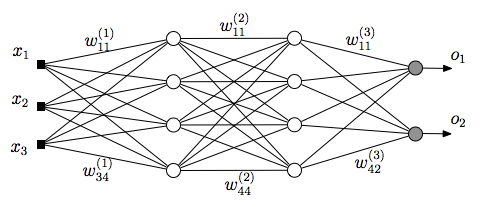
\includegraphics[scale=0.5]{img/MLP}
%     \caption{Paveikslėlio pavyzdys}   % Antraštė įterpiama po paveikslėlio
%     \label{img:mlp}
% \end{figure}


% \section{Eksperimentinio palyginimo rezultatai}
% % tablesgenerator.com - converts calculators (e.g. excel) tables to LaTeX
% \begin{table}[H]\footnotesize
%   \centering
%   \caption{Lentelės pavyzdys}    % Antraštė įterpiama prieš lentelę
%   {\begin{tabular}{|l|c|c|} \hline
%     Algoritmas & $\bar{x}$ & $\sigma^{2}$ \\
%     \hline
%     Algoritmas A  & 1.6335    & 0.5584       \\
%     Algoritmas B  & 1.7395    & 0.5647       \\
%     \hline
%   \end{tabular}}
%   \label{tab:table example}
% \end{table}

\end{document}
